\chapter{SYSTEM DESIGN}
\begin{spacing}{1.2}
\minitoc
\thispagestyle{MyStyle}
\end{spacing}
\newpage

\section{INTRODUCTION}
This chapter presents the technical design of the SIPMS platform. We detail the overall system architecture, the class model with all entities and their relationships, the sequence diagrams for key workflows, and the relational database schema.

\section{GENERAL ARCHITECTURE}

\subsection{Architectural Pattern}
SIPMS follows a \textbf{client-server architecture} with a clear separation of concerns across three tiers:

\begin{itemize}[leftmargin=2cm, topsep=0pt]
    \begin{spacing}{1.25}
        \item \textbf{Presentation Layer}: A React (Vite) single-page application running in the browser, communicating with the backend exclusively via RESTful HTTP requests.
        \item \textbf{Business Logic Layer}: A Spring Boot application exposing a secured REST API, organized into Controllers, Services, and Repositories following the layered architecture pattern.
        \item \textbf{Data Layer}: A MySQL 8 relational database accessed via Spring Data JPA (Hibernate), with schema managed through entity definitions.
    \end{spacing}
\end{itemize}

\begin{figure}[H]
    \centering
    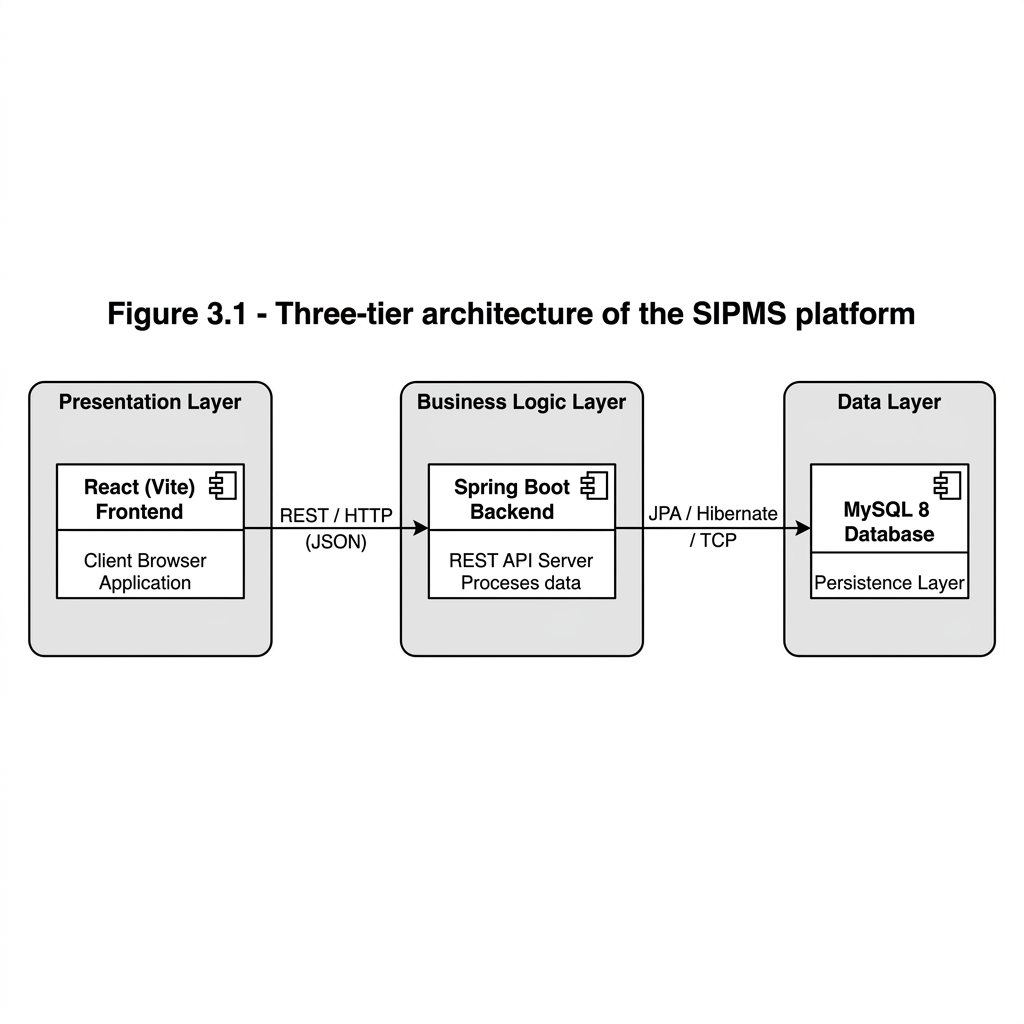
\includegraphics[width=\textwidth]{images/TemplateImages/three_tier_architecture.png}
    \caption{Three-tier architecture of the SIPMS platform}
    \label{fig:three-tier}
\end{figure}

\subsection{Backend Package Structure}
The Spring Boot backend is organized into the following packages:

\begin{table}[H]
\centering
\begin{tabular}{|p{4.5cm}|p{8.5cm}|}
\hline
\rowcolor{gray!20}
\textbf{Package} & \textbf{Responsibility} \\
\hline
\texttt{controller} & Exposes REST endpoints; handles HTTP requests and responses \\
\hline
\texttt{service} & Contains business logic; orchestrates between controllers and repositories \\
\hline
\texttt{repository} & Spring Data JPA interfaces for database access \\
\hline
\texttt{entity} & JPA entity classes mapped to database tables \\
\hline
\texttt{dto} & Data Transfer Objects for request/response payloads \\
\hline
\texttt{security} & JWT filter, authentication entry point, Spring Security configuration \\
\hline
\texttt{common} & Shared utilities: ApiResponse wrapper, FileStorageService, AuditService \\
\hline
\texttt{ai} & AI scoring and matching engine \\
\hline
\end{tabular}
\caption{Backend package structure}
\end{table}

\subsection{Security Architecture}
Authentication in SIPMS is stateless and JWT-based. The security flow operates as follows:

\begin{enumerate}
    \item The client sends credentials (email + password) to \texttt{POST /api/auth/login}.
    \item Spring Security validates credentials via \texttt{UserDetailsService} and BCrypt.
    \item On success, a signed JWT token (HS512) is generated and returned to the client.
    \item For subsequent requests, the client includes the token in the \texttt{Authorization: Bearer} header.
    \item The \texttt{JwtAuthenticationFilter} intercepts every request, validates the token signature and expiration, and populates the \texttt{SecurityContext}.
    \item \texttt{@PreAuthorize} annotations on controller methods enforce role-based access.
\end{enumerate}

\section{CLASS DIAGRAM}

\subsection{Core Entity Relationships}
The domain model consists of 16 entities organised into three subsystems: Core Domain, Quiz Subsystem, and AI Subsystem. The class diagram is decomposed into subsystems to enhance readability and maintain modularity. Each entity corresponds directly to a database table and is involved in at least one use case scenario defined in Chapter 2.

\subsubsection{Core Domain Subsystem}
The core domain subsystem includes the primary business entities that handle authentication, candidate management, applications, and supervision:

\begin{table}[H]
\centering
\small
\begin{tabular}{|p{2.5cm}|p{4cm}|p{6.5cm}|}
\hline
\rowcolor{gray!20}
\textbf{Entity} & \textbf{Key Attributes} & \textbf{Relationships} \\
\hline
\textbf{User} & id, firstName, lastName, email, passwordHash, phone, cin, avatarUrl, active, mustChangePassword, specialty, internshipYear, status, quizScore, createdAt, updatedAt & ManyToMany $\rightarrow$ Role; OneToOne $\leftarrow$ Candidate (optional); OneToMany $\rightarrow$ Notification; OneToMany $\rightarrow$ AuditLog; OneToMany $\rightarrow$ Document (uploadedBy) \\
\hline
\textbf{Role} & id, name (ADMIN, MANAGER, RECEPTIONIST, CANDIDATE) & ManyToMany $\leftarrow$ User \\
\hline
\textbf{Candidate} & id, firstName, lastName, email, phone, cin, assignedQuizId, createdAt, updatedAt & OneToOne $\rightarrow$ User (optional); OneToMany $\rightarrow$ InternshipFile (EAGER); OneToMany $\rightarrow$ Application; OneToMany $\rightarrow$ QuizAttempt; OneToMany $\rightarrow$ Interview \\
\hline
\textbf{InternshipFile} & id, year, university, degree, skillsTags, createdAt, updatedAt & ManyToOne $\rightarrow$ Candidate; OneToMany $\rightarrow$ Document \\
\hline
\textbf{Document} & id, fileName, filePath, fileType, fileSize, documentType (CV, COVER\_LETTER, TRANSCRIPT, ID\_CARD, PHOTO, OTHER), createdAt & ManyToOne $\rightarrow$ Application (optional); ManyToOne $\rightarrow$ InternshipFile (optional); ManyToOne $\rightarrow$ User (uploadedBy) \\
\hline
\textbf{Application} & id, intakeMethod (ONLINE, PHYSICAL), status (8-state DFA), managerNotes, aiMatchScore, decisionDate, createdAt, updatedAt & ManyToOne $\rightarrow$ Candidate (EAGER); ManyToOne $\rightarrow$ Project; ManyToOne $\rightarrow$ Supervisor; ManyToOne $\rightarrow$ User (registeredBy) \\
\hline
\textbf{Supervisor} & id, fullName, email, department, expertiseTags, maxInterns (default 3), currentInterns, bio, active, createdAt & OneToOne $\rightarrow$ User; OneToMany $\rightarrow$ Project; OneToMany $\rightarrow$ Application \\
\hline
\textbf{Project} & id, title, description, domain, technologyTags, requiredSkills, aiScore, status (DRAFT, SUBMITTED, APPROVED, REJECTED), createdAt, updatedAt & ManyToOne $\rightarrow$ User (submittedBy); ManyToOne $\rightarrow$ Supervisor \\
\hline
\textbf{Interview} & id, scheduledAt, interviewer, type (TECHNICAL/HR), status (SCHEDULED/COMPLETED/CANCELLED), score, notes, feedback, createdAt, updatedAt & ManyToOne $\rightarrow$ Candidate; ManyToOne $\rightarrow$ Application \\
\hline
\textbf{Notification} & id, title, message, type (INFO/SUCCESS/WARNING/ERROR), isRead, link, createdAt & ManyToOne $\rightarrow$ User \\
\hline
\textbf{AuditLog} & id, action, entityType, entityId, details, ipAddress, createdAt & ManyToOne $\rightarrow$ User \\
\hline
\end{tabular}
\caption{Core domain subsystem entities}
\end{table}

\subsubsection{Quiz Subsystem}
The quiz subsystem manages assessment creation, question banks, and candidate attempt tracking:

\begin{table}[H]
\centering
\small
\begin{tabular}{|p{2.5cm}|p{4cm}|p{6.5cm}|}
\hline
\rowcolor{gray!20}
\textbf{Entity} & \textbf{Key Attributes} & \textbf{Relationships} \\
\hline
\textbf{Quiz} & id, title, description, durationMins (default 30), passingScore (default 60), totalMarks (default 100), specialty, active, createdAt & ManyToOne $\rightarrow$ User (createdBy); OneToMany $\rightarrow$ QuizQuestion; OneToMany $\rightarrow$ QuizAttempt \\
\hline
\textbf{QuizQuestion} & id, questionText, optionA, optionB, optionC, optionD, correctOption (A/B/C/D), marks (default 5), orderIndex & ManyToOne $\rightarrow$ Quiz \\
\hline
\textbf{QuizAttempt} & id, score, totalMarks, percentage, passed, startedAt, completedAt & ManyToOne $\rightarrow$ Quiz; ManyToOne $\rightarrow$ Candidate; ManyToOne $\rightarrow$ Application; OneToMany $\rightarrow$ QuizAnswer \\
\hline
\end{tabular}
\caption{Quiz subsystem entities}
\end{table}

\subsubsection{AI Subsystem}
The AI subsystem stores the outputs of intelligent ranking and matching operations:

\begin{table}[H]
\centering
\small
\begin{tabular}{|p{2.5cm}|p{4cm}|p{6.5cm}|}
\hline
\rowcolor{gray!20}
\textbf{Entity} & \textbf{Key Attributes} & \textbf{Relationships} \\
\hline
\textbf{AiRanking} & id, rankingType (PROJECT\_RANK, CANDIDATE\_MATCH), referenceId, score (0.0--1.0), reasoning (AI explanation text), createdAt & ManyToOne $\rightarrow$ Supervisor (optional); ManyToOne $\rightarrow$ User (rankedBy) \\
\hline
\end{tabular}
\caption{AI subsystem entities}
\end{table}

\subsection{Relationship Diagram}
The key relationships between entities are summarized as follows:

\begin{verbatim}
User *-- Role (ManyToMany)
Candidate "1" --> "0..1" User (optional OneToOne)
Candidate "1" *--> "0..*" InternshipFile (OneToMany, EAGER)
InternshipFile "1" *--> "0..*" Document (OneToMany)
Application "1" --> "0..*" Document (OneToMany)
Candidate "1" *--> "0..*" Application (OneToMany)
Application "1" --> "0..1" Project (ManyToOne)
Application "1" --> "0..1" Supervisor (ManyToOne)
Application "1" --> "0..1" User (registeredBy)
Supervisor "1" *--> "0..*" Project (OneToMany)
Supervisor "1" --> "0..1" User (OneToOne)
Quiz "1" *--> "0..*" QuizQuestion (OneToMany)
Quiz "1" *--> "0..*" QuizAttempt (OneToMany)
Candidate "1" *--> "0..*" QuizAttempt (OneToMany)
Application "1" *--> "0..*" QuizAttempt (OneToMany)
Candidate "1" *--> "0..*" Interview (OneToMany)
Application "1" *--> "0..*" Interview (OneToMany)
User "1" *--> "0..*" Quiz (createdBy)
User "1" *--> "0..*" Notification (OneToMany)
User "1" *--> "0..*" AuditLog (OneToMany)
Supervisor "1" --> "0..*" AiRanking (OneToMany)
User "1" --> "0..*" AiRanking (rankedBy)
\end{verbatim}

Beyond data-level entity relationships, the system also defines the following \texttt{<<include>>} and \texttt{<<extend>>} relationships between use cases, capturing functional dependencies and optional extensions:

\begin{verbatim}
--- Include Relationships (mandatory) ---
Login                  <<include>>   Complete Assigned Quiz
Login                  <<include>>   Register Candidate
Login                  <<include>>   Upload CV for AI Analysis
Complete Assigned Quiz <<include>>   Generate AI Ranking
Complete Assigned Quiz <<include>>   Schedule Interview
Generate AI Ranking    <<include>>   Assign Supervisor to Candidate

--- Extend Relationships (optional) ---
Register Candidate     <<extend>>    Upload CV for AI Analysis
Complete Assigned Quiz <<extend>>    Send Automated Email Notification
Update Application     <<extend>>    Send Automated Email Notification
Schedule Interview     <<extend>>    Send Automated Email Notification
\end{verbatim}

\begin{figure}[H]
    \centering
    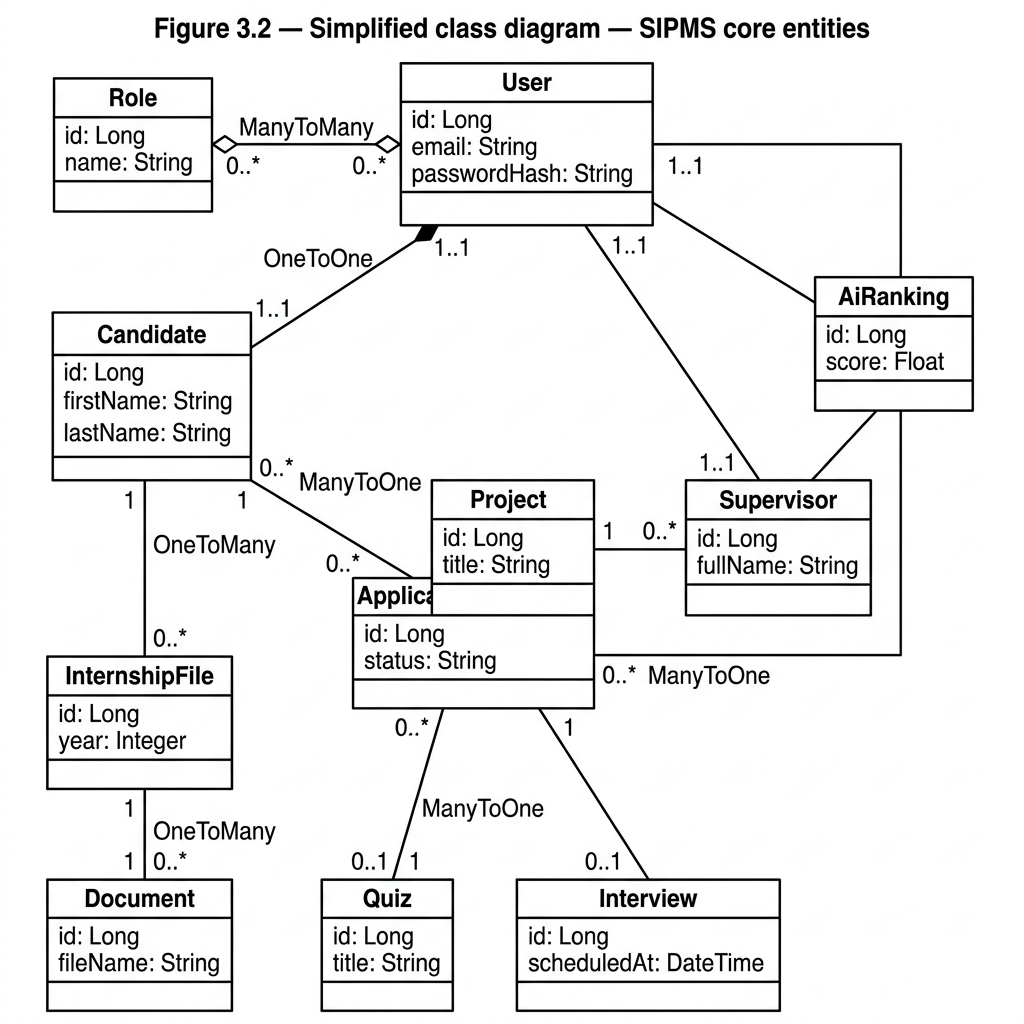
\includegraphics[width=\textwidth]{images/TemplateImages/simplified_class_diagram.png}
    \caption{Simplified class diagram --- SIPMS core entities}
    \label{fig:class-diagram}
\end{figure}

\subsection{Entity Interaction and Call Flow}
The class diagram defines the static structure, but the dynamic behavior is governed by how these entities call one another during runtime. The key interaction flows are as follows:

\renewcommand{\labelitemi}{\tiny$\bullet$}
\begin{itemize}[leftmargin=2cm, topsep=4pt]
    \begin{spacing}{1.25}
        \item \textbf{Authentication flow}: \texttt{User} $\rightarrow$ \texttt{Role} (via ManyToMany). The \texttt{JwtAuthenticationFilter} reads the authenticated \texttt{User}'s roles from the \texttt{SecurityContext} and enforces access via \texttt{@PreAuthorize} annotations on controller methods.
        \item \textbf{Candidate registration flow}: \texttt{Frontend} $\rightarrow$ \texttt{CandidateController} $\rightarrow$ \texttt{CandidateService} $\rightarrow$ \texttt{CandidateRepository} saves a new \texttt{Candidate}. The optional \texttt{User} entity is NOT created at this stage — it is created later during the manager approval step (\texttt{approveAndSendQuiz()}), which establishes the OneToOne link from \texttt{Candidate} to \texttt{User}.
        \item \textbf{Internship file upload flow}: \texttt{Frontend} $\rightarrow$ \texttt{CandidateController} $\rightarrow$ \texttt{CandidateService} $\rightarrow$ \texttt{InternshipFileRepository} saves the \texttt{InternshipFile} linked to the \texttt{Candidate}. If a document is attached, \texttt{FileStorageService} writes the file to disk, then a \texttt{Document} entity is created and added to the \texttt{InternshipFile}'s documents collection.
        \item \textbf{Quiz assignment and evaluation flow}: \texttt{Manager} approves candidate $\rightarrow$ \texttt{CandidateService.approveAndSendQuiz()} $\rightarrow$ creates \texttt{User} (optional OneToOne), reads or creates \texttt{Quiz}, creates \texttt{QuizAttempt} linking \texttt{Candidate}, \texttt{Quiz}, and \texttt{Application}. When the candidate submits answers, \texttt{QuizService} grades them, persists \texttt{QuizAnswer} records, updates \texttt{QuizAttempt.score/percentage/passed}, and advances the \texttt{Application.status}.
        \item \textbf{Interview scheduling flow}: \texttt{Manager} $\rightarrow$ \texttt{InterviewController} $\rightarrow$ \texttt{InterviewService} $\rightarrow$ saves \texttt{Interview} with references to \texttt{Candidate} and \texttt{Application}. When the result is recorded, \texttt{Interview.score}, \texttt{Interview.notes}, and \texttt{Interview.feedback} are updated, and the \texttt{Interview.status} transitions from \texttt{SCHEDULED} to \texttt{COMPLETED}.
        \item \textbf{AI evaluation flow}: \texttt{Manager} triggers AI matching $\rightarrow$ \texttt{AiService} $\rightarrow$ reads \texttt{Candidate}'s skills (via \texttt{InternshipFile.skillsTags}), quiz performance (\texttt{QuizAttempt.percentage}), and project requirements (\texttt{Project.domain}, \texttt{Project.technologyTags}). The weighted score is computed and persisted as an \texttt{AiRanking} record linked to the \texttt{Supervisor}. The \texttt{Application.aiMatchScore} field is also updated for quick reference on the manager dashboard.
    \end{spacing}
\end{itemize}

\subsection{AI Entities and Scoring Logic}
The AI module introduces two specialized concepts that are embedded across multiple entities:

\subsubsection{AI Scoring Fields}
AI-generated scores are stored directly on existing entities to avoid joins and simplify queries:

\begin{itemize}[leftmargin=2cm, topsep=4pt]
    \begin{spacing}{1.25}
        \item \textbf{Application.aiMatchScore} (Double): A value between 0.0 and 1.0 representing the AI's confidence that the candidate is a good fit for the assigned project. Calculated by analyzing the candidate's quiz score (\texttt{QuizAttempt.percentage}), skills tags (\texttt{InternshipFile.skillsTags}), and degree level against the project's domain and technology requirements.
        \item \textbf{Project.aiScore} (Double): A value between 0.0 and 1.0 representing the overall quality and relevance score of a project proposal. Calculated based on description completeness, domain alignment with company priorities, and the submitting candidate's profile strength.
    \end{spacing}
\end{itemize}

\subsubsection{AiRanking Entity}
The \texttt{AiRanking} entity stores the output of AI-based ranking operations:

\begin{itemize}[leftmargin=2cm, topsep=4pt]
    \begin{spacing}{1.25}
        \item \textbf{rankingType}: An enum with two values — \texttt{PROJECT\_RANK} (ranks projects by relevance for a given candidate) and \texttt{CANDIDATE\_MATCH} (ranks candidates by suitability for a given supervisor).
        \item \textbf{referenceId}: The ID of the ranked entity (project ID for PROJECT\_RANK, candidate ID for CANDIDATE\_MATCH).
        \item \textbf{score}: A Double between 0.0 and 1.0 representing the AI's confidence score.
        \item \textbf{reasoning}: A free-text field containing the AI's natural language explanation of the score. Example: \textit{"Candidate has strong Java and Spring Boot skills matching the supervisor's expertise. Quiz score of 85\% indicates solid technical foundation."}
        \item \textbf{supervisor}: Optional ManyToOne to Supervisor. Present only when the ranking is a CANDIDATE\_MATCH targeting a specific supervisor.
        \item \textbf{rankedBy}: The User (Admin/Manager) who triggered the AI evaluation.
    \end{spacing}
\end{itemize}

\subsubsection{AI Scoring Algorithm}
The AI scoring follows a weighted formula:

\begin{verbatim}
AI Match Score = w1 x skillOverlap + w2 x quizPerformance + w3 x academicLevel

Where:
  skillOverlap    = |candidateSkills and projectSkills| / |projectSkills|
  quizPerformance = QuizAttempt.percentage / 100
  academicLevel   = degreeLevel / maxDegreeLevel

Default weights: w1=0.40, w2=0.40, w3=0.20
\end{verbatim}

These scores are computed by the \texttt{AiService} which delegates to the configured AI provider (GPT-4-mini) for the reasoning generation, while the numerical scoring uses deterministic formulas for consistency and reproducibility.

\section{SEQUENCE DIAGRAMS}

Five sequence diagrams are presented in this section to illustrate the dynamic behaviour of the SIPMS platform. Each diagram corresponds to one or more use cases defined in Chapter 2 and models the interactions between actors, frontend components, backend services, and the database.

\subsection{Sequence: Candidate Registration with Internship File Upload}
This sequence describes the complete candidate registration and document upload flow performed by the receptionist. It corresponds to the use cases \textbf{Register a New Candidate} and \textbf{Add Internship File with Document}.

\begin{enumerate}
    \item The receptionist fills the candidate form (firstName, lastName, email, phone, CIN) and submits it via the React frontend.
    \item The frontend calls \texttt{POST /api/candidates} with the candidate data as a JSON payload.
    \item \texttt{CandidateService.createCandidate()} validates the input, persists the \texttt{Candidate} entity to the database, and returns the created record with its generated identifier.
    \item The receptionist then opens the internship file form and enters the year, university, degree, and skills tags. Optionally, a PDF document may be attached.
    \item The frontend calls \texttt{POST /api/candidates/\{id\}/internship-files/with-document} using multipart form data to transmit both the metadata and the uploaded file.
    \item \texttt{FileStorageService.storeFile()} saves the uploaded document to \texttt{./uploads/candidates/\{id\}/} with a UUID-based filename to prevent path traversal and naming collisions.
    \item An \texttt{InternshipFile} entity is persisted and linked to the candidate. If a file was uploaded, a \texttt{Document} entity is also persisted and associated with the \texttt{InternshipFile}.
    \item The frontend refreshes the candidates table and the internship files list to reflect the newly added data.
\end{enumerate}

\begin{figure}[H]
    \centering
    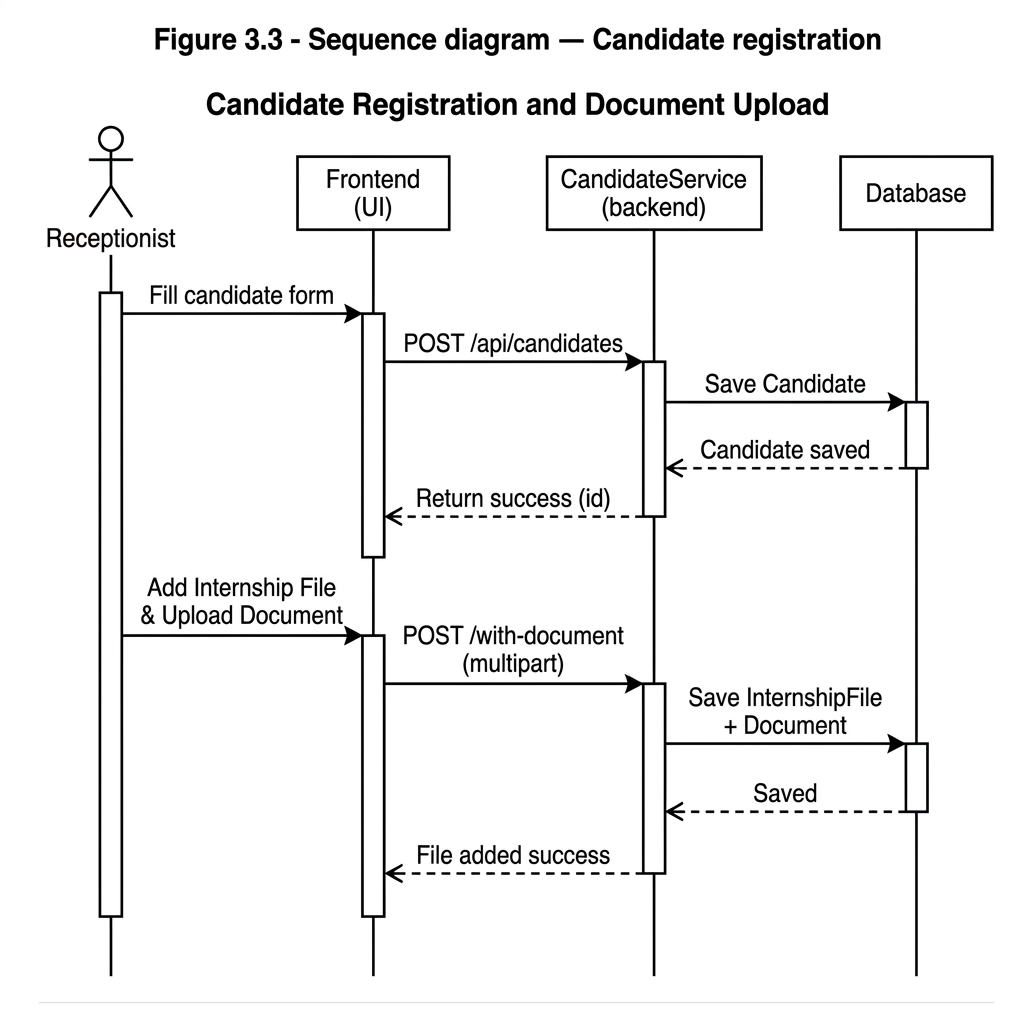
\includegraphics[width=\textwidth]{images/TemplateImages/sequence_candidate_registration.png}
    \caption{Sequence diagram --- Candidate registration with document upload}
    \label{fig:sequence-registration}
\end{figure}

\subsection{Sequence: Approve Candidate and Send Quiz}
This sequence corresponds to the use case \textbf{Approve and Send Quiz} (User Story US-18) and models the manager's approval workflow.

\begin{enumerate}
    \item The manager selects a candidate from the candidates table and clicks "Approve \& Send Quiz".
    \item The \texttt{QuizSelectionModal} opens and loads existing quizzes via \texttt{GET /api/quizzes} for the manager to choose from.
    \item The manager either selects an existing quiz from the list or opts to create a default 5-question MCQ quiz.
    \item The frontend calls \texttt{POST /api/candidates/\{id\}/approve-and-send-quiz} with an optional \texttt{quizId} in the request body.
    \item \texttt{CandidateService.approveAndSendQuiz()} performs the following steps transactionally:
        \begin{enumerate}
            \item Creates a \texttt{User} account for the candidate with a BCrypt-hashed temporary password and sets the \texttt{mustChangePassword} flag.
            \item If a \texttt{quizId} was provided, creates a \texttt{QuizAttempt} linking the candidate to the existing quiz.
            \item If no \texttt{quizId} was provided, creates a new \texttt{Quiz} containing 5 default MCQs, then creates the corresponding \texttt{QuizAttempt}.
            \item Sends an HTML email via Gmail SMTP containing the candidate's login credentials and the assigned quiz title.
        \end{enumerate}
    \item The frontend refreshes the candidates view, displaying the candidate with an active user account and an assigned quiz status.
\end{enumerate}

\subsection{Sequence: Interview Scheduling and Result Recording}
This sequence corresponds to the use cases \textbf{Schedule Interview} and \textbf{Record Interview Result} (User Stories US-19 and US-20).

\begin{enumerate}
    \item The manager identifies a candidate whose application is in \texttt{QUIZ\_COMPLETED} status and who has passed the quiz (\texttt{passed = true}).
    \item The manager clicks "Schedule Interview" and fills the scheduling form with a date and time, interviewer name, and interview type (TECHNICAL or HR).
    \item The frontend calls \texttt{POST /api/interviews} with the candidate identifier, application identifier, scheduled timestamp, interviewer, and type.
    \item \texttt{InterviewService.createInterview()} validates the scheduling constraints and persists the interview with status \texttt{SCHEDULED}.
    \item The newly scheduled interview appears in the interview management page alongside existing records.
    \item After the interview takes place, the manager records the result by calling \texttt{PUT /api/interviews/\{id\}/result} with the score, notes, and feedback. The service updates the interview status to \texttt{COMPLETED} and persists the evaluation data.
\end{enumerate}

\section{DATABASE SCHEMA}

\subsection{Main Tables}
\begin{table}[H]
\centering
\small
\begin{tabular}{|p{3cm}|p{10cm}|}
\hline
\rowcolor{gray!20}
\textbf{Table} & \textbf{Key Columns} \\
\hline
\texttt{users} & id, first\_name, last\_name, email, password\_hash, phone, cin, avatar\_url, active, must\_change\_password, specialty, internship\_year, status, quiz\_score, quiz\_created\_at, quiz\_completed\_at, created\_at, updated\_at \\
\hline
\texttt{roles} & id, name (ADMIN, MANAGER, RECEPTIONIST, CANDIDATE) \\
\hline
\texttt{user\_roles} & user\_id, role\_id \\
\hline
\texttt{candidates} & id, first\_name, last\_name, email, phone, cin, assigned\_quiz\_id, user\_id (nullable FK), created\_at, updated\_at \\
\hline
\texttt{internship\_files} & id, candidate\_id (FK), year, university, degree, skills\_tags, created\_at, updated\_at \\
\hline
\texttt{documents} & id, application\_id (nullable FK), internship\_file\_id (nullable FK), uploaded\_by (FK), file\_name, file\_path, file\_type, file\_size, document\_type (CV, COVER\_LETTER, TRANSCRIPT, ID\_CARD, PHOTO, OTHER), created\_at \\
\hline
\texttt{applications} & id, candidate\_id (FK), project\_id (FK), supervisor\_id (FK), registered\_by (FK), intake\_method (ONLINE, PHYSICAL), status (PENDING..REJECTED), manager\_notes, decision\_date, ai\_match\_score, created\_at, updated\_at \\
\hline
\texttt{supervisors} & id, user\_id (FK), full\_name, email, department, expertise\_tags, max\_interns, current\_interns, bio, active, created\_at \\
\hline
\texttt{projects} & id, title, description, domain, technology\_tags, required\_skills, status (DRAFT, SUBMITTED, APPROVED, REJECTED), ai\_score, submitted\_by (FK), supervisor\_id (FK), created\_at, updated\_at \\
\hline
\texttt{quizzes} & id, title, description, duration\_mins, passing\_score, total\_marks, specialty, active, created\_by (FK), created\_at \\
\hline
\texttt{quiz\_questions} & id, quiz\_id (FK), question\_text, option\_a, option\_b, option\_c, option\_d, correct\_option, marks, order\_index \\
\hline
\texttt{quiz\_attempts} & id, quiz\_id (FK), candidate\_id (FK), application\_id (FK), score, total\_marks, percentage, passed, started\_at, completed\_at \\
\hline
\texttt{quiz\_answers} & id, attempt\_id (FK), question\_id (FK), selected\_option, is\_correct \\
\hline
\texttt{interviews} & id, candidate\_id (FK), application\_id (FK), scheduled\_at, interviewer, type (TECHNICAL, HR), status (SCHEDULED, COMPLETED, CANCELLED), score, notes, feedback, created\_at, updated\_at \\
\hline
\texttt{notifications} & id, user\_id (FK), title, message, type (INFO, SUCCESS, WARNING, ERROR), is\_read, link, created\_at \\
\hline
\texttt{audit\_log} & id, user\_id (FK), action, entity\_type, entity\_id, details, ip\_address, created\_at \\
\hline
\texttt{ai\_rankings} & id, ranking\_type (PROJECT\_RANK, CANDIDATE\_MATCH), reference\_id, score, reasoning, supervisor\_id (FK), ranked\_by (FK), created\_at \\
\hline
\end{tabular}
\caption{Complete database schema (17 tables)}
\end{table}

\subsection{Normalization Analysis}
The database schema is designed to comply with \textbf{Third Normal Form (3NF)} to minimize data redundancy and ensure referential integrity:

\begin{itemize}[leftmargin=2cm, topsep=4pt]
    \begin{spacing}{1.25}
        \item \textbf{First Normal Form (1NF)}: All tables have a single-column primary key (\texttt{id}) with auto-increment. Every column contains atomic values — for example, \texttt{skills\_tags} stores comma-separated tags as a single string (denormalized for simplicity), while multi-valued attributes like quiz options use separate columns (\texttt{option\_a}, \texttt{option\_b}, etc.) rather than arrays or JSON.
        \item \textbf{Second Normal Form (2NF)}: All non-key columns are fully functionally dependent on the primary key. There are no partial dependencies because every table uses a single-column primary key. For example, \texttt{documents.file\_name} depends only on \texttt{documents.id}, not on any candidate or application attribute.
        \item \textbf{Third Normal Form (3NF)}: No transitive dependencies exist. Every non-key column depends directly on the primary key, not on another non-key column. For instance, \texttt{quizzes.passing\_score} depends only on \texttt{quizzes.id}, not on \texttt{quizzes.specialty} or \texttt{quizzes.title}.
    \end{spacing}
\end{itemize}

Small controlled denormalizations were intentionally applied for performance:
\begin{itemize}[leftmargin=2cm, topsep=4pt]
    \begin{spacing}{1.25}
        \item \textbf{Application.aiMatchScore} and \textbf{Project.aiScore} are stored directly on the entity rather than in a separate scores table, avoiding a join on every dashboard load.
        \item \textbf{InternshipFile.skillsTags} uses a comma-separated string rather than a junction table, since tags are small in number and always retrieved together with the file record.
    \end{spacing}
\end{itemize}

\subsection{Constraints and Integrity Rules}
The schema enforces the following constraints to guarantee data quality:

\begin{itemize}[leftmargin=2cm, topsep=4pt]
    \begin{spacing}{1.25}
        \item \textbf{NOT NULL constraints} on all business-critical columns: \texttt{users.email}, \texttt{candidates.email}, \texttt{internship\_files.year}, \texttt{applications.status}, \texttt{interviews.scheduled\_at}, \texttt{documents.file\_name}.
        \item \textbf{UNIQUE constraints}: \texttt{users.email} is unique to prevent duplicate accounts. \texttt{candidates.email} is also unique to prevent duplicate registrations.
        \item \textbf{CHECK constraints} enforced via Java enums mapped to MySQL ENUM columns: \texttt{applications.status} (PENDING, UNDER\_REVIEW, QUIZ\_PENDING, QUIZ\_COMPLETED, AI\_EVALUATING, MANAGER\_REVIEW, ACCEPTED, REJECTED), \texttt{interviews.type} (TECHNICAL, HR), \texttt{documents.document\_type} (CV, COVER\_LETTER, TRANSCRIPT, ID\_CARD, PHOTO, OTHER).
        \item \textbf{DEFAULT values}: \texttt{applications.status} defaults to \texttt{PENDING}, \texttt{interviews.status} defaults to \texttt{SCHEDULED}, \texttt{quizzes.active} defaults to \texttt{true}.
        \item \textbf{CASCADE rules}: Deleting a \texttt{Candidate} cascades to all linked \texttt{InternshipFile} and \texttt{Application} records. Deleting an \texttt{InternshipFile} cascades to its \texttt{Document} records.
        \item \textbf{Foreign key constraints}: Every \texttt{FOREIGN KEY} ensures that referenced records exist. For example, \texttt{internship\_files.candidate\_id} references \texttt{candidates.id} and prevents orphaned records.
    \end{spacing}
\end{itemize}

\subsection{Schema Design Decisions}
The relational schema follows the entity relationships described in Section 3.3. Foreign key constraints enforce referential integrity across all tables. Key design decisions include:

\begin{itemize}[leftmargin=2cm, topsep=0pt]
    \begin{spacing}{1.25}
        \item \textbf{Nullable foreign keys}: \texttt{documents.application\_id} and \texttt{documents.internship\_file\_id} are both nullable because a document can belong to either an application or an internship file, but not necessarily both.
        \item \textbf{Optional User link}: \texttt{candidates.user\_id} is nullable because a candidate exists independently of a User account. The User is created only when the manager invites/approves the candidate.
        \item \textbf{Enum types}: Status fields (application status, interview status, document type) are stored as MySQL ENUM types for data integrity.
        \item \textbf{Audit timestamps}: All entities include \texttt{created\_at} and most include \texttt{updated\_at}, populated automatically via JPA's \texttt{@PrePersist} and \texttt{@PreUpdate} hooks.
    \end{spacing}
\end{itemize}

\subsection{Diagram Quality and Formal Coherence}
The UML diagrams presented in this chapter adhere to standard modeling conventions and maintain formal coherence across all levels of abstraction. The following quality criteria were applied:

\renewcommand{\labelitemi}{\tiny$\bullet$}
\begin{itemize}[leftmargin=2cm, topsep=4pt]
    \begin{spacing}{1.25}
        \item \textbf{UML compliance}: Class diagrams follow UML 2.5 notation with correct multiplicity markers (\texttt{1}, \texttt{0..*}, \texttt{0..1}), directed associations for foreign key relationships, and diamond-free aggregation since all relationships are standard associations with explicit JPA annotations. Associations are annotated with fetch types (EAGER vs LAZY) and cascade behaviors where relevant.
        \item \textbf{Cross-diagram traceability}: Every entity in the class diagram participates in at least one sequence diagram interaction. For example, the \texttt{Candidate} entity appears in the registration sequence, the quiz sequence, and the interview sequence. Each sequence diagram, in turn, corresponds to a specific use case described in Chapter 2, ensuring end-to-end traceability from requirements to design.
        \item \textbf{Subsystem consistency}: The decomposition into Core Domain, Quiz, and AI subsystems in the class diagram aligns with the five functional modules defined in the system decomposition (Chapter 2). Entities within each subsystem have cohesive responsibilities and minimal cross-subsystem dependencies, reducing coupling and improving maintainability.
        \item \textbf{Entity-to-table mapping}: Each class diagram entity maps directly to a MySQL database table via JPA \texttt{@Entity} and \texttt{@Table} annotations. Field-level \texttt{@Column} mappings define column names, nullability, lengths, and constraints, ensuring database schema coherence with the domain model. This one-to-one mapping eliminates impedance mismatch between the object-oriented and relational representations.
        \item \textbf{Behavioral consistency}: Sequence diagrams model the dynamic behavior of the system in a way that is consistent with the static structure defined in the class diagram. Lifelines correspond to controller, service, and entity instances derived from the class model, while messages map to method calls on those instances. The state machine for application lifecycle transitions is consistent with the status field defined on the \texttt{Application} entity, and every valid transition corresponds to a guard condition enforced in the service layer.
        \item \textbf{Normalization and denormalization balance}: The schema achieves 3NF for transactional data while applying controlled denormalizations (\texttt{Application.aiMatchScore}, \texttt{InternshipFile.skillsTags}) for performance-critical read paths, as detailed in Section 3.5.3. This balance ensures data integrity without sacrificing query performance.
    \end{spacing}
\end{itemize}

\section{CONCLUSION}
This chapter presented the complete technical design of SIPMS, covering the three-tier client-server architecture, the JWT-based stateless security model with HS512 signing and BCrypt password hashing, and the full class diagram decomposed into three subsystems (Core Domain with 11 entities, Quiz subsystem with 3 entities, and AI subsystem). The entity-relationship diagram and use case include/extend dependencies were formalised to ensure traceability between the static structure and dynamic behaviour of the system. Five sequence diagrams illustrated the key workflows — authentication, candidate registration, quiz approval and completion, interview scheduling, and CV analysis — each consistent with the use cases defined in Chapter 2. The database schema was presented with 17 tables, normalised to 3NF with controlled denormalisations for performance, and enforced through foreign key, unique, check, and cascade constraints. These design decisions provide a solid blueprint for the implementation phase described in the next chapter.
